% !TeX TS-program = lualatex
\documentclass[12pt,letterpaper]{article}
%%% LuaLaTex
\usepackage{fontspec}
\usepackage[spanish,mexico]{babel}
\usepackage{amsmath}% if desired
\usepackage{unicode-math}
\renewcommand{\boldsymbol}{\symbf}

\setmainfont{TeX Gyre Pagella}[
Numbers	=	{OldStyle, Proportional},
Ligatures	=	TeX,
%Script=Arabic
%Contextuals = WordFinal,	
]
\setsansfont{TeX Gyre Adventor}[
Numbers	=	{OldStyle, Proportional},
Ligatures	=	TeX,
Scale=MatchLowercase]
\setmonofont{Inconsolata}[
Scale = MatchLowercase, 
Ligatures = TeX,
]
\setmathfont{Asana Math}
\setmathfont[range=it->up]{Neo Euler}
\setmathfont[range=up/{num}]{Neo Euler}
\newfontface{\andm}{Andale Mono}
\newfontface{\babm}{BabelStone Mayan Numerals}%{Symbola}
\newfontface{\mayanumerals}{BabelStone Mayan Numerals}
\newfontface{\charis}{Charis SIL}%{Gentium Plus}
\newfontface{\charisbf}{Charis SIL Bold}%{Charis SIL}
%\newfontface{\palarab}{PalatinoLTArabic}%{Gentium Plus}
%%%%%%%%%%%%
\linespread{1.05}% Palatino needs more leading (space between lines) {1.01} {1.08}
%\usepackage{ucs}

%\usepackage{amsmath}
%\usepackage{amsfonts}
%\usepackage{amssymb}
%\usepackage{makeidx}
\usepackage[format=hang,font=small,labelfont=bf,labelsep=quad]{caption}
\usepackage{xcolor}
\usepackage{graphicx}
\usepackage[useregional]{datetime2}
\usepackage{fancyhdr}
\usepackage{tikz}
\usepackage[colorlinks=true,urlcolor=brown]{hyperref}
% % % %Geometry
\usepackage{geometry}%\usepackage[showframe]{geometry}
%\usepackage{layout}
\setlength{\voffset}{-0.7in}
\setlength{\headsep}{10pt}
\setlength{\textheight}{10.5in}
\usepackage{wasysym} %emoticons :)
%\usepackage[oldstyle]{kpfonts}
%\usepackage[T1]{fontenc}
\newcommand{\LuaLaTeX}{L\kern-0.25em\raise0.5ex\hbox{\tiny U}\kern-0.04em\raise0.5ex\hbox{\tiny A}\kern-0.05em\LaTeX}
\newcommand{\fej}{\relax\hfill\ifmmode{\lower.5ex\hbox{{\textcolor{blue}{\LARGE\smiley al 15pt}}}}\else\lower.5ex\hbox{{\textcolor{blue}{\LARGE \smiley}}}}  % Smiley emoticon :)
\author{\textsc{Manuel López Mateos}}
%%% Nov 3, 2019
% % % % % % % Para usar título, autor y fecha por separado.
\makeatletter
\let\newtitle\@title
\let\elautor\@author
\let\newdate\@date
\makeatother
%
%
% % % % Enviroments
\newenvironment{definition}[1][Definición.]{\begin{trivlist}
\item[\hskip \labelsep {\bfseries #1}]}{\end{trivlist}}
% % % % % % % % % % % %
%
% % % % % % % % Headers
\pagestyle{fancy}
\fancyhf{}
\rhead{\color{olive}\hfill \DTMnow}
\lhead{\color{olive}\elautor}
\cfoot{\thepage}
\renewcommand{\headrule}{\color{olive}\hrule}
\newcommand{\R}{\relax\ifmmode\mathbb{R}\else${\mathbb{R}}$\fi}
%\rfoot{}
% % % % % % %
\begin{document} %\layout
%\noindent{\color{purple} \elautor \hfill \DTMnow
%\smallskip
%
%\hrule}
\bigskip 

\noindent Encuentra la ecuación de la  \emph{\color{purple}mediatriz} del lado $\overline{BC}$ en el triángulo definido por los puntos $A=(-2,4)$, $B=(-3,-2)$ y $C=(6,-1)$.
\medskip

Las \textbf{\color{purple}mediatrices} de un triángulo son las rectas que perpendiculares al punto medio de cada lado. Así, la \emph{mediatriz} de $\overline{BC}$, debe ser perpendicular a la recta que contiene al segmento $\overline{BC}$ y debe pasar por el punto medio $D$ del \emph{segmento} $\overline{BC}$, según se muestra en la figura. 
\begin{figure}[ht]
\centering
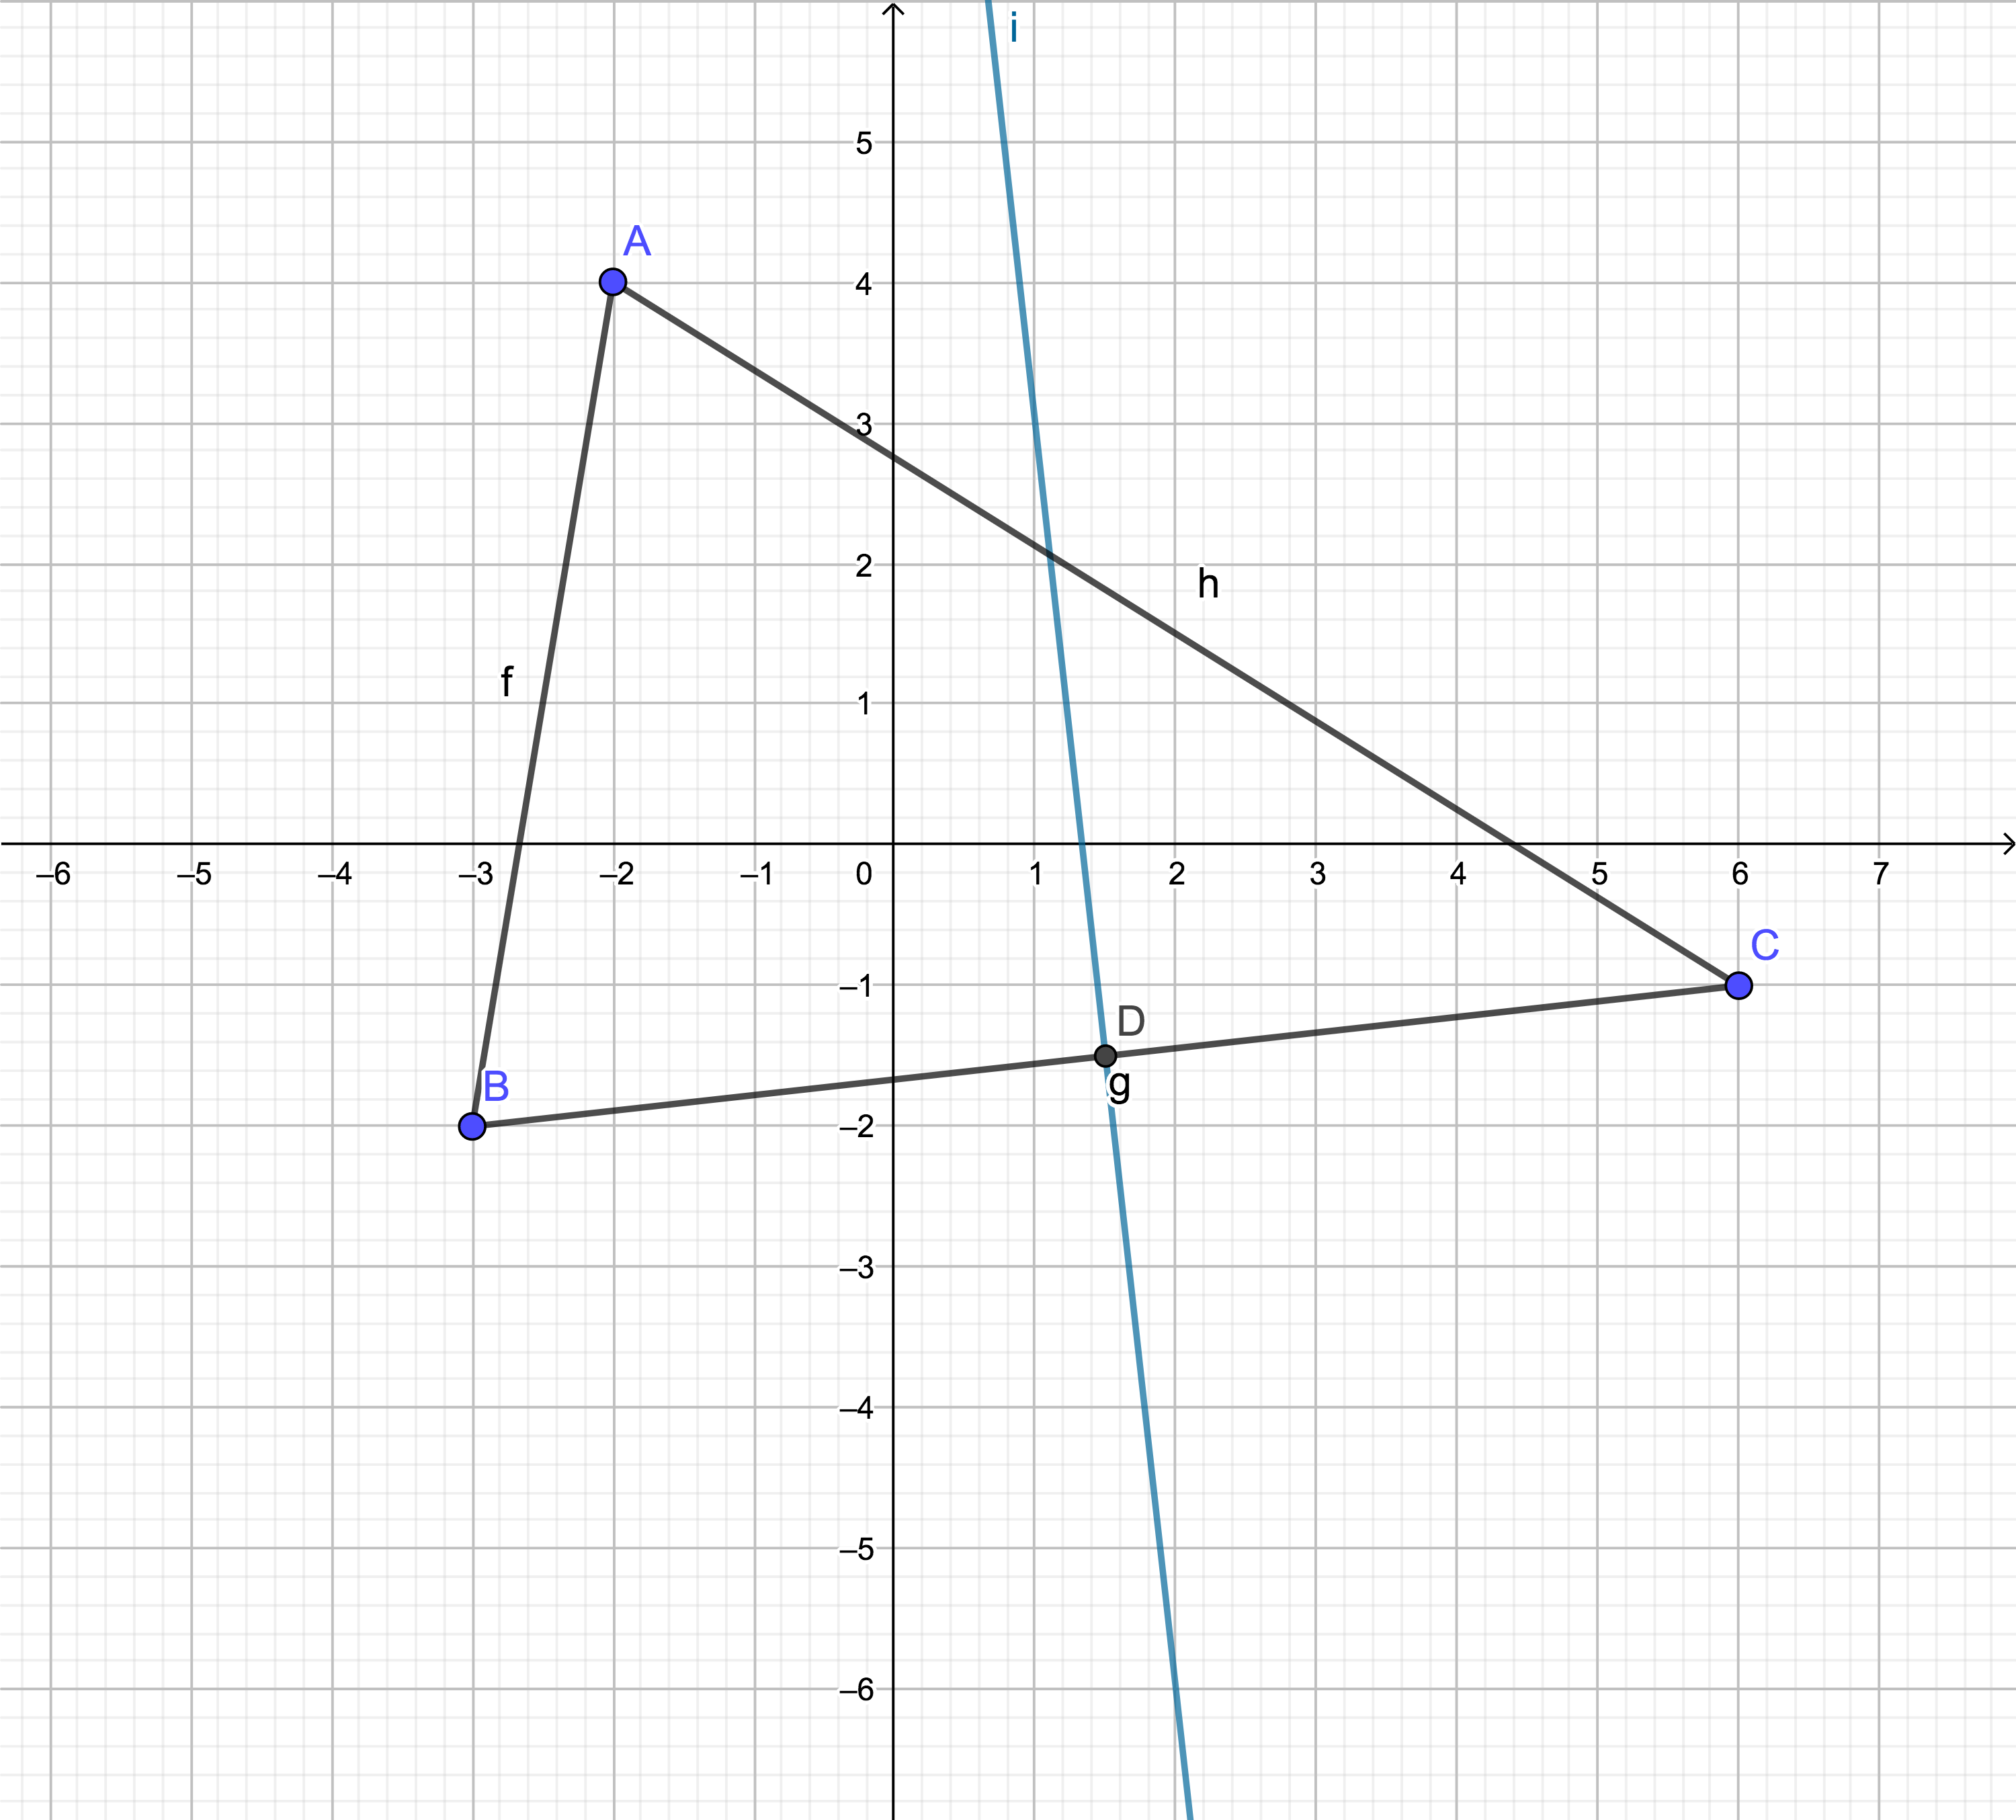
\includegraphics[scale=0.31]{img/mediatriz-triang.png}
\caption{La mediatriz de $\overline{BC}$, es la perpendicular a $\overline{BC}$ que pasa por el punto medio $D$.}\label{fig:mediatriz}
\end{figure}

Las \emph{tres} mediatrices se \emph{\color{purple}intersecan} en un punto, llamado \textbf{\color{purple}circuncentro} del triángulo.

Las coordenadas del punto medio $D$ del segmento $\overline{BC}$ son las \emph{\color{purple}medias aritméticas} de las coordenadas de los extremos del segmento, de $B$ y de $C$,
\begin{equation*}
D=(d_1,d_2)=\left(\frac{-3+6}{2},\frac{-2+(-1)}{2}\right) =\left(\frac{3}{2},-\frac{3}{2}\right).
\end{equation*} 

Si una recta $L$ tiene pendiente $m_1$, cualquier recta perpendicular a $L$ tiene pendiente $m_2$ tal que $m_1m_2=-1$.

La pendiente $m_1$ de la recta que pasa por los puntos $B$ y $C$ es la razón de los incrementos $\Delta y$ y $\Delta x$,
\begin{equation*}
\Delta y = -1-(-2) = 1\,,\qquad
\Delta x = 6-(-3) = 9\,,
\end{equation*}
y
$$m_1=\frac{\Delta y}{\Delta x} =  \frac{1}{9}.$$
Luego $m_2=-9$, pues $-9\cdot\dfrac{1}{9}=-1$.

La forma canónica de la ecuación de la mediatriz es
$$y=-9x+b.$$
Para hallar $b$, substituimos en la ecuación anterior las coordenadas de $D$,
$$-\frac{3}{2}=-9\frac{3}{2}+b,\quad\text{de donde}\quad b=-\frac{3}{2}`+\frac{27}{2}=12.$$
Así, la ecuación buscada de la mediatriz, en su forma canónica, es
\[y=-9x+12.\tag*{\fej}\]

Verifica que la forma general de la ecuación es $-9x-y+12=0$.

¿Puedes encontrar el \textbf{\color{purple}circuncentro del triángulo?}






\vfill 

\begin{center}
	{\footnotesize\color{olive} Hoja formada con \LuaLaTeX. La gráfica con \textsc{Geogebra}, \url{https://www.geogebra.org/m/kvbbv6vc/}}
\end{center}
\end{document}